%\begin{flushright}
%%%\emph{``For the things we have to learn before we can do them, we learn by doing them.''}\\%Each wrong scenario you have analysed, is a wrong decision you won't made.''}\\
%%%Aristote
%\emph{All models are wrong, but some are useful.}\\
%George P. Box
%\end{flushright}

%\medskip
%
%\begin{mybox}{Chapter overview}
%\begin{itemize}[left=0em]%[leftmargin=0cm,itemindent=.5cm,labelwidth=\itemindent,labelsep=0cm,align=left]
%\setlength\itemsep{-0.3em}
%\item Belgian energy system overview%Case studies: the Belgian energy systems during the transition (2015-2050).
%\end{itemize}
%\vspace{-0.3cm}
%
%\emph{This chapter is an improved and extended case study version of \citet{Limpens_belgian_2020}}.
%\end{mybox}
%
%\medskip

As detailed by \citet{limpens2024pathway}, the analysis carried out in this work can be applied to any regional whole-energy system. As a densely-populated and highly-industrialised country with limited local renewable potentials (mainly solar and wind), the transition of Belgium from a fossil-dominated system in 2020 (Appendix \ref{app:bel_2020}) to carbon-neutrality in 2050 makes it an intricate case study. Moreover, this case study and the subsequent analyses can be transferred - to some extent - to other industrialised countries highly dependent on fossil fuels with limited local renewable potentials (\eg the Netherlands or Germany) \cite{dommisse2020modelling}. This chapter presents the different demands to satisfy, with a particular focus on the non-energy demand, as well as the resources available and the conversion technologies to supply those. For a comprehensive understanding and detailed descriptions of the technologies, please refer to the documentation \cite{readthedocs_pathway}. Then, the uncertainty ranges considered for some of the parameters are detailed. Finally, the \ce{CO2}-budget over the 2020-2050 transition is presented.

\section*{Contributions}
\label{sec:cs:contributions}
First, as pointed out by \citet{rixhon2022integration}, where most of the studies assessing whole-energy system integrate energy demands (\ie electricity, heart and mobility), the \gls{NED} is often not considered. The latter is defined as ‘\textit{energy products used as raw materials in the different sectors; that is not consumed as a fuel or transformed into another fuel}’ \cite{Eurostat2019}. The previous analyses carried out with \gls{ESTD} considered the non-energy demand as the related primary energy needs, \ie either natural gas or \gls{LFO}. To minimise the total cost of the system, the model simply selected the cheapest between the two resources (\ie natural gas). This work goes one step further and accounts for the \gls{NED} as a demand of three commodities (\ie \gls{HVC}, ammonia and methanol) as well as with associated production technologies. This allows bringing the non-energy sector to a similar level of details as the other sectors.  Regarding the end-use demands,  keeping the same methodology to define \gls{EUD} in EnergyScope as \citet{Limpens2020}, this work considers updated values given the latest release of the \og EU reference scenario 2020 : energy, transport and GHG emissions: Trends to 2050 \fg by the European Commission \cite{EuropeanCommission2021}.\\

Second, given the focus of this work on the electrofuels, the case study includes a more explicit representation of e-ammonia and e-methanol (as well as their fossil-based equivalents), on top of e-hydrogen and e-methane, already included in the previous definition of the case study \cite{limpens2021generating}. As detailed later on, these electrofuels are considered as renewable in the sense that their \gls{GWP} is zero. This more explicit representation of the molecules themselves also comes with a more exhaustive integration of the ways to produce and use them in the system.\\

Third, as nuclear energy could be a real game-changer in the energy transition worldwide \cite{IEA2022nuclear}, and especially in Belgium, this thesis has integrated the potential to install \gls{SMR} from 2040 onward.\\

Fourth, where previous works considered a prescribed \ce{CO2} trajectory to reach carbon-neutrality by 2050 \cite{limpens2021generating, limpens2024pathway}, the case study analysed in this thesis is subject to a \ce{CO2}-budget for the transition, \ie limiting the total amount of emissions over the transition.\\

Finally, to a smaller extent, this work includes updated values for some parameters compared to the work of \citet{limpens2021generating}. The main change concerns the cost and performance of private mobility vehicles, which is specifically a key components in the Belgian energy transition. The previous version of the case study was excessively favouring fuel cell car versus \gls{BEV}. Comparing with other works \cite{schnidrig2021modelling, EuropeanCommission2021}, the CAPEX and efficiency of fuel cell cars have been increased. Regarding \gls{BEV}, while the CAPEX has been kept unchanged, the efficiency and the battery capacity, \ie the range, have been increased. As seen in the results, this change of data made \gls{BEV} often more competitive than its hydrogen-based equivalent. 

\section{End-use demands}
\label{sec:cs:demand}
End-use demands, exogenously imposed as inputs to the model, are characterised by yearly quantities to satisfy and are also distributed over the different hours of each representative years of the transition, in order to account for their daily or seasonal variability \cite{Limpens2020,limpens2021generating}. In this work, the yearly end-use demands (EUD) for all sectors are calculated from the rather slightly increasing forecast proposed by the European Commission for Belgium (Appendix 2 in report \cite{EuropeanCommission2021}). 

\subsection{Non-energy demand}
\label{subsec:cs:NED}
Where previously published works of \citet{rixhon2021comprehensive,rixhon2022integration} investigated more extensively the integration of the \gls{NED} in the case study of Belgium, this section summarises the rationale of doing so as well as the methodology used to quantify this demand.\\

\vspace{0.2cm}\textbf{Definition and historical trend}\vspace{-0.3cm}\\

The \gls{NED} can be split into four main categories of final molecules \cite{IEA2018_petrochemicals}: (i) \gls{HVC} (worldwide production of $\sim$365Mt/year); (ii) ammonia ($\sim$185Mt/year); (iii) methanol ($\sim$100Mt/year) and (iv) the other products. \Gls{HVC} gather the light olefins (e.g. ethylene, propylene) and aromatics (benzene, toluene, xylene – BTX), mainly for the production of plastics, synthetic fibers or rubber. Their production today relies mainly on petroleum products such as naphtha, ethane or liquified petroleum gas. Ammonia is  mainly used for the production of fertilizers ($\sim$80\% of global ammonia consumption). Its production is dominated by \gls{NG} via steam reforming to produce hydrogen, used as feedstock in the Haber-Bosch process. Methanol is mainly converted to formaldehyde (resin) but also used for the production of other chemicals (e.g. solvents and gasoline-blends). Currently, its synthesis, like ammonia, is mainly relying on natural gas via steam reforming. Finally, the other products gather all chemicals not mentioned in the other categories such as bitumen, lubricants and other heavy products from oil refineries \cite{daioglou2014energy}.\\

The \gls{NED} currently represents around 20\% of the final energy consumption in Belgium \cite{FPSEconomy2021}. Over the recent history, there has been a relatively constant evolution of three main categories of the final consumption for non-energy use in Belgium, \cite{statbel_NED_2019}: (i) naphtha and \gls{LPG} (between 59\% and 67\% of the total final consumption, around 59.4\,TWh in 2019), (ii) \gls{NG} (between 9\% and 14\%, 11.8\,TWh in 2019), and (iii) others (\ie bitumen, coal tar and other oil products) (between 21\% and 28\%). Naphtha and \gls{LPG} are consumed in a naphtha cracker, which results in ethylene and propylene, what will be considered as \gls{HVC} in the rest of this work. Similarly, \gls{NG}, as non-energy carrier, is used in steam methane reformer to produce the required hydrogen to the synthesis process of ammonia. The small shares of bitumen and coal tar are respectively used for roadworks and to produce synthetic gas through gasification. Finally \og other oil products\fg take into account, indistinguishably, tar and sulphur as well as by-products of the refineries (\eg \gls{BTX}). About methanol, there is currently no production plant in Belgium even if the country plays a role in trading this commodity between its neighbouring countries and consumes part of what it imports.\\

\vspace{0.2cm}\textbf{Methodology of quantification}\vspace{-0.3cm}\\

The non-energy demand studied in this analysis focuses on the chemical industry (more than 90\% of the non-energy use in Belgium) and, similarly to other studies \cite{IEA2018_petrochemicals, daioglou2014energy}, is split between the three aforementioned main groups of products (\ie \gls{HVC}, ammonia and methanol). Before describing these three demands, this study excludes bitumen, coal tar and \og other oil products\fg. The first two represent marginal shares of the current non-energy use in such a way that they should not affect the big trends provided by this study. As described previously, the latest are mostly by-products from refineries that the system uses because they are available. However, in a perspective of defossilisation, since the future of fossil-based refineries is unclear, they have not be implemented in this study nor their by-products.\\

Regarding \gls{HVC}, the future of their production is highly uncertain. One of the reasons is new regulations and strategies promoting recycling and limitation of single-use plastics \cite{EU_plastics}.  Besides this uncertainty, Belgium stays a major exporter as approximately 2/3 of plastic raw materials produced locally are exported abroad \cite{agoria_plastics}. Even if a significant part of \gls{HVC} produced in Belgium is not locally consumed, this demand has been set based on the assumption that Belgium will keep its industrial activity in this sector. This assumption does not consider the net imports of \gls{HVC}, unlike ammonia and methanol, which will be more traded commodities in the future (as energy carriers and non-energy products). Therefore, the actual demand of \gls{HVC} is inferred from the consumption of naphtha and \gls{LPG} as non-energy use as well as energy-carrier in the chemical and petrochemical industries \cite{statbel_NED_2019}. This assumption is based on the fact that, in the conversion processes to produce \gls{HVC} from naphtha or \gls{LPG}, these fuels also serve as energy-carrier to supply the process itself. Then, given the respective efficiencies (1.83t$_{\text{naphtha}}$/t$_{\text{HVC}}$ and 1.67t$_{\text{LPG}}$/t$_{\text{HVC}}$) \cite{IEA2018_petrochemicals}, the current demand of \gls{HVC} is estimated equal to 3069\,kt, without making distinctions between the different chemicals (\ie ethylene, propylene and \gls{BTX}). \\

The ammonia sector in Belgium is quite different: the country locally produces and imports ammonia much more than it exports it. Thanks to a database from the United Nations \cite{UN_statistics} and the National Bank of Belgium, it has been identified that, over the last ten years, Belgium has imported, exported and locally produced, on average, respectively, 1010\,kt, 105\,kt and 990\,kt of ammonia. Therefore, on top of the local production, the net import (\ie import minus export) is also included in this non-energy demand. This gives a current demand of 1895\,kt of ammonia.\\

Concerning the demand of methanol, similarly to ammonia, this work solely considers the net imports as there is no local production in Belgium. To define the actual non-energy demand of methanol, only a 51\%-share of this net import is kept since, according to the Methanol Institute and \gls{MMSA}, this share is used for formaldehyde production in Belgium \cite{MMSA51}. The rest of the methanol is used for energy purposes, mostly as \gls{MTBE} in gasoline blending. This methodology gives a current non-energy demand of methanol of 269\,kt.\\

Finally, after converting these masses of products into energy content (\ie LHV: \gls{HVC} - 47\,MJ/kg, ammonia - 18.8\,MJ/kg and methanol - 19.9\,MJ/kg), this work assumed constant shares between the three categories within the \gls{NED} and the same growing rate as presented by \citet{EuropeanCommission2016}.

\subsection{Forecast of the demands over the transition}
\label{subsec:cs:EUD_forecast}
Although, given a significant and unsubstantiated discrepancy in the non-energy use forecasts compared to their previous report (\ie +80\% over the 2020-2030 time window), the evolution trend of the \gls{NED} of the current work has been inferred from the previous edition, published in 2016, \cite{EuropeanCommission2016}. Looking at \Cref{fig:cs_demands}, between 2020 and 2050, one observes a noteworthy increase of the electricity (+40\%), passenger (+45\%) and freight mobility (+35\%) demands. The rise of the non-energy demand is more limited, \ie +6\%, whereas the heating demands is forecast to decrease: -11\% and -3\% respectively for the low and high-temperature heat demands. Regarding the center graph of \Cref{fig:cs_demands}, it is the aggregation of the same data as in the left graph but per category, rather than per sector, with the non-energy demand being associated with the industry. This illustrates how industrialised is Belgium, compared to households and services, and, consequently, highly energy-intensive. The right graph of \Cref{fig:cs_demands} gives the passenger and the freight mobility. The sharp increase from 2020 to 2025 is due the COVID-crisis that has significantly reduced these demands in 2020. As far as the hourly discretisation of these demands is concerned, time series are based on historical values of 2015 for parts of electricity and low-temperature heating demands \cite{Limpens2020}. A daily time series is used for the passenger mobility and applied similarly to every typical days. Finally, for the other demands, the yearly demand is distributed uniformly over the different hours of the year.

\begin{figure}[htbp!]
\centering
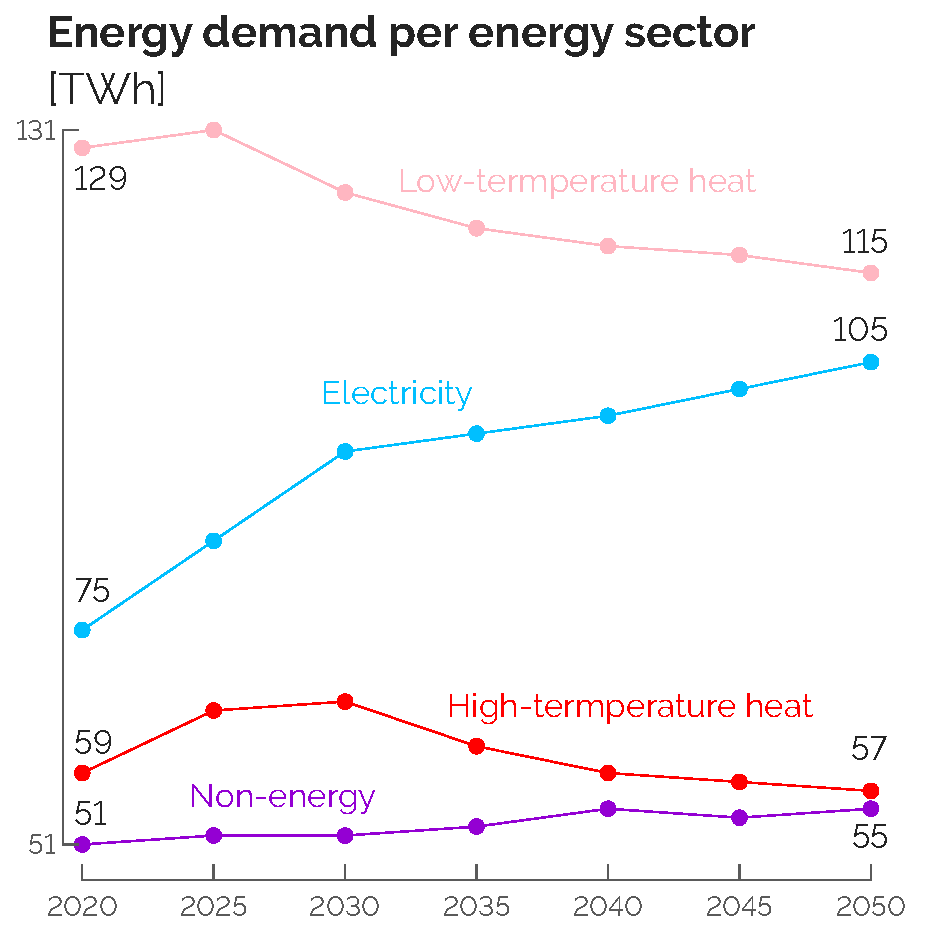
\includegraphics[width=0.32\textwidth]{EUD_sec.pdf}
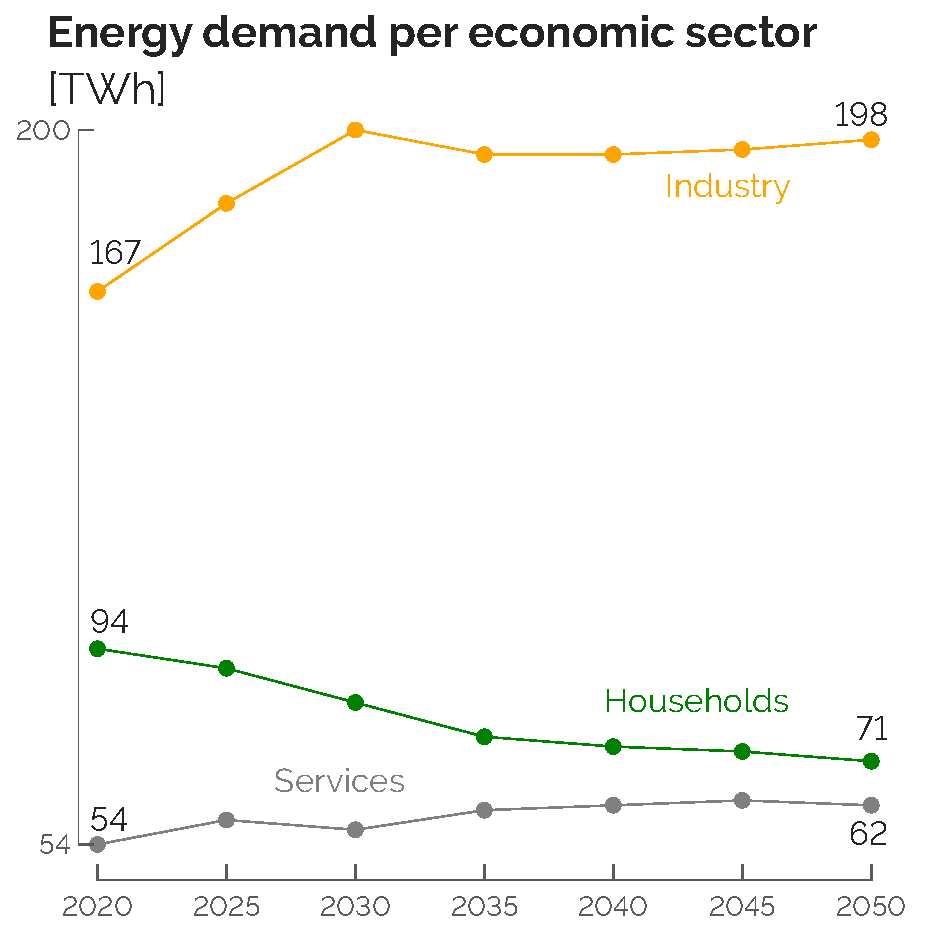
\includegraphics[width=0.32\textwidth]{EUD_cat.pdf}
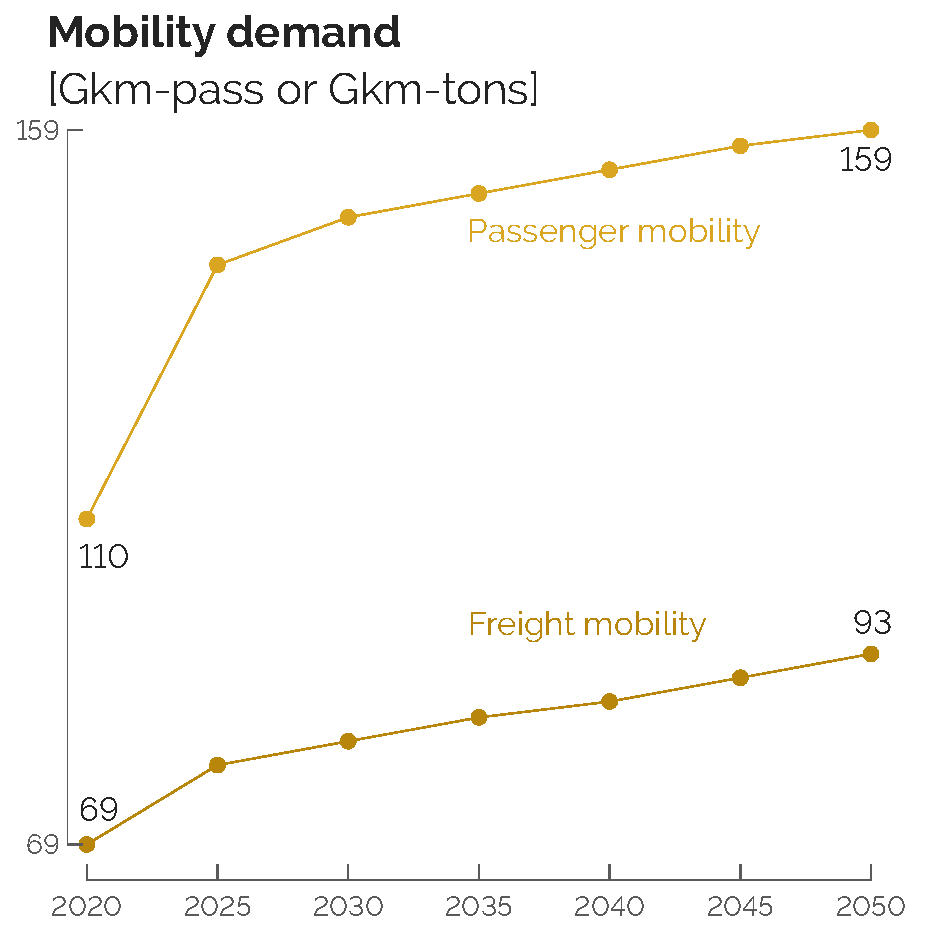
\includegraphics[width=0.32\textwidth]{EUD_mob.pdf}
\caption{EnergyScope splits the whole-energy system end-use demands (EUD) into two sets: (non)-energy and transport-related. This figure presents the nominal values of each of these demands. In the center graph, the non-energy demand has been fully associated with the industrial demand. As detailed previously, the non-energy demand is expressed in tons of physical products (\ie \glsxtrfull{HVC}, ammonia and methanol) and then translated into their respective energy equivalent, in TWh. Graphs have been adapted from \cite{limpens2024pathway}.}
\label{fig:cs_demands}
\end{figure}


\section{Resources}
\label{sec:cs:resources}
To supply the aforementioned demands, EnergyScope Pathway implements a variety of resources defined by their cost of purchasing, $\mathit{c}_{\mathrm{op}}$, their global warming potential, $\mathit{gwp}_{\mathrm{op}}$, as well as their 
availability, as detailed by \citet{limpens2024pathway}. \Cref{fig:cs_resources_cost} depicts the evolution the respective costs of purchasing. Regarding ``renewable electrofuels'', these are in line with the recent study of \citet{genge2023supply} who carried out an extensive review and ``meta-analysis\cite{grant2009typology,page2021prisma} of 30 studies on the supply costs of chemical energy carriers''. Then, besides their cost, the resources are either limited or unlimited in terms of availability and either renewable or not. The limitation in terms of availability can be direct or indirect. On the one hand, woody (23.4\,TWh) and wet biomass (38.9\,TWh) are limited by their local potentials and the consumption of waste (17.8\,TWh) and coal (33.4\,TWh) is assumed not to exceed the current use. On the other hand, wind, solar, hydro and uranium are limited by the technical potentials respectively, of \gls{PV} panels (59.2\,GW), onshore (10\,GW) and offshore (6\,GW) wind turbines, run-of-the-river power plants (0.1\,GW) and nuclear power plants (6\,GW). As \gls{SMR} are foreseen, if installed, to be around the same locations (\ie Thiange and Doel) as the conventional nuclear power plants and using the same area in kW/ha, the same 6\,GW are assumed to be the maximum capacity for \gls{SMR}. This is even without considering the potential limit due to the local availability, in terms of volume and flow rate, of enough water that would be a more socially-accepted solution than cooling towers exhausting a dense plume. Imported electricity is limited in two ways: the potential of instantaneous capacity of interconnection with neighbouring countries (\ie 11.9\,GW by 2050 \cite{ELIA_2050}) and a limitation to 30\% of the yearly electricity end-use demand (\ie 32.4\,TWh by 2050). In the current work, the electrofuels (\ie e-methane, e-hydrogen, e-methanol and e-ammonia) are assumed to be ``sustainable" in the sense that they do not increase the concentration of \ce{CO2} in the atmosphere \cite{rixhon2021terminology}. In practice, it means that their \gls{GWP} is assumed to be zero in the model. Regarding specifically these electrofuels, the \citet{h2coalition} has carried out an extensive techno-economic analysis to estimate their respective cost of purchasing, after having identified some key locations from which importing these energy carriers (\eg Chile, Australia or Morocco). As the amount to import from each of these locations is hard to forecast, the current work considers the average cost between the different locations. Besides these, every other resource has its specific \gls{GWP} like coal ($\mathit{gwp}_{\mathrm{op,coal}}=0.40$\,kt$_{\ce{CO2},\text{eq}}$/GWh), natural gas ($\mathit{gwp}_{\mathrm{op,NG}}=0.27$\,kt$_{\ce{CO2},\text{eq}}$/GWh) or the fossil-based molecules equivalent to the electrofuels (\eg $\mathit{gwp}_{\mathrm{op,ammonia}}=0.46$\,kt$_{\ce{CO2},\text{eq}}$/GWh or $\mathit{gwp}_{\mathrm{op,methanol}}=0.41$\,kt$_{\ce{CO2},\text{eq}}$/GWh).

\begin{figure}[htbp!]
\centering

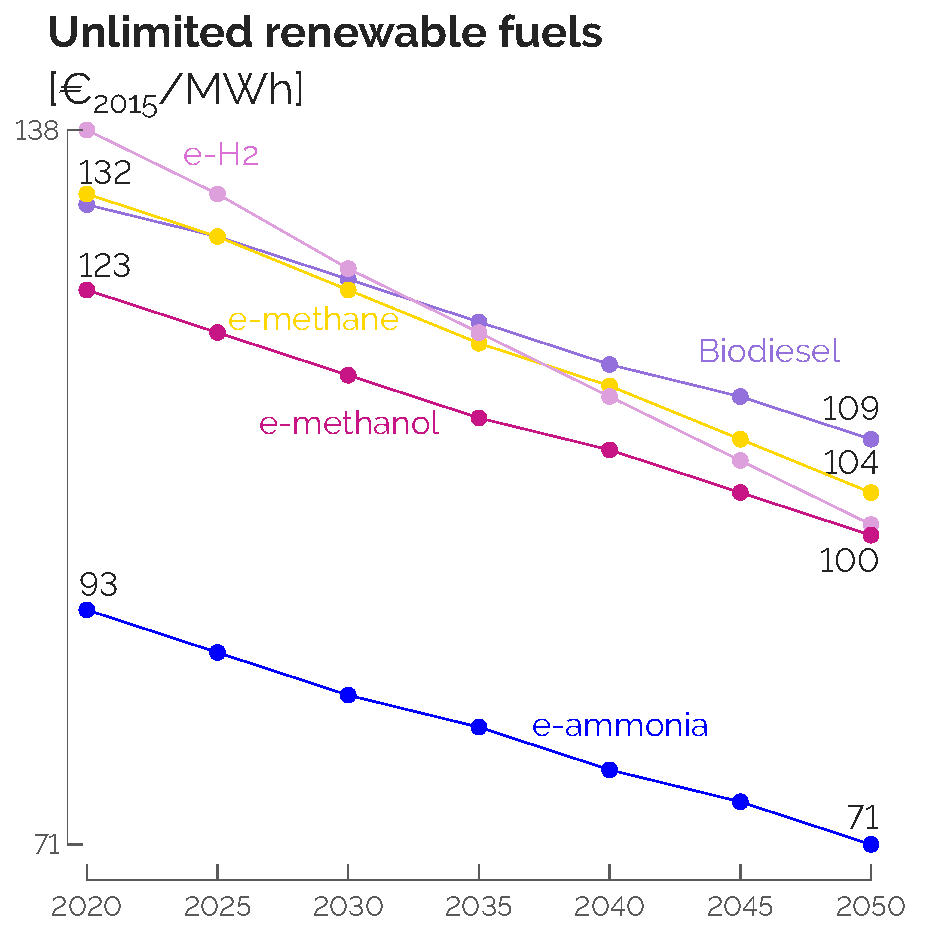
\includegraphics[width=0.32\textwidth]{Res_ren.pdf}
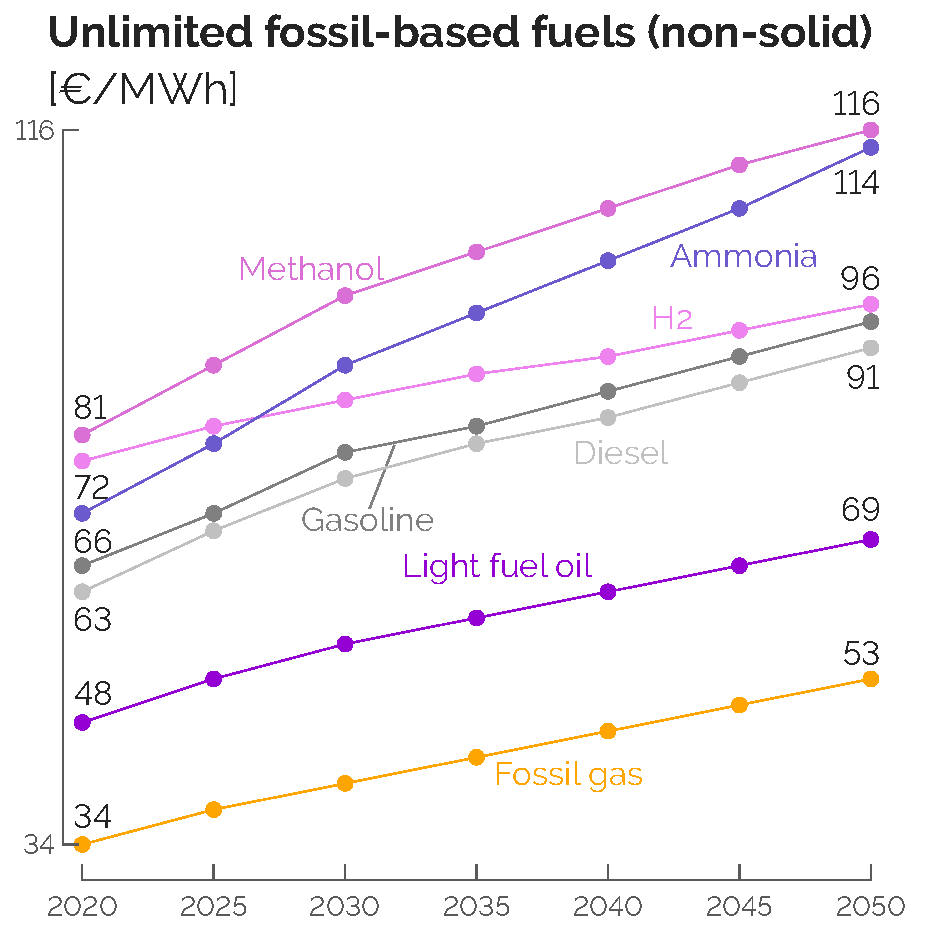
\includegraphics[width=0.32\textwidth]{Res_foss.pdf}
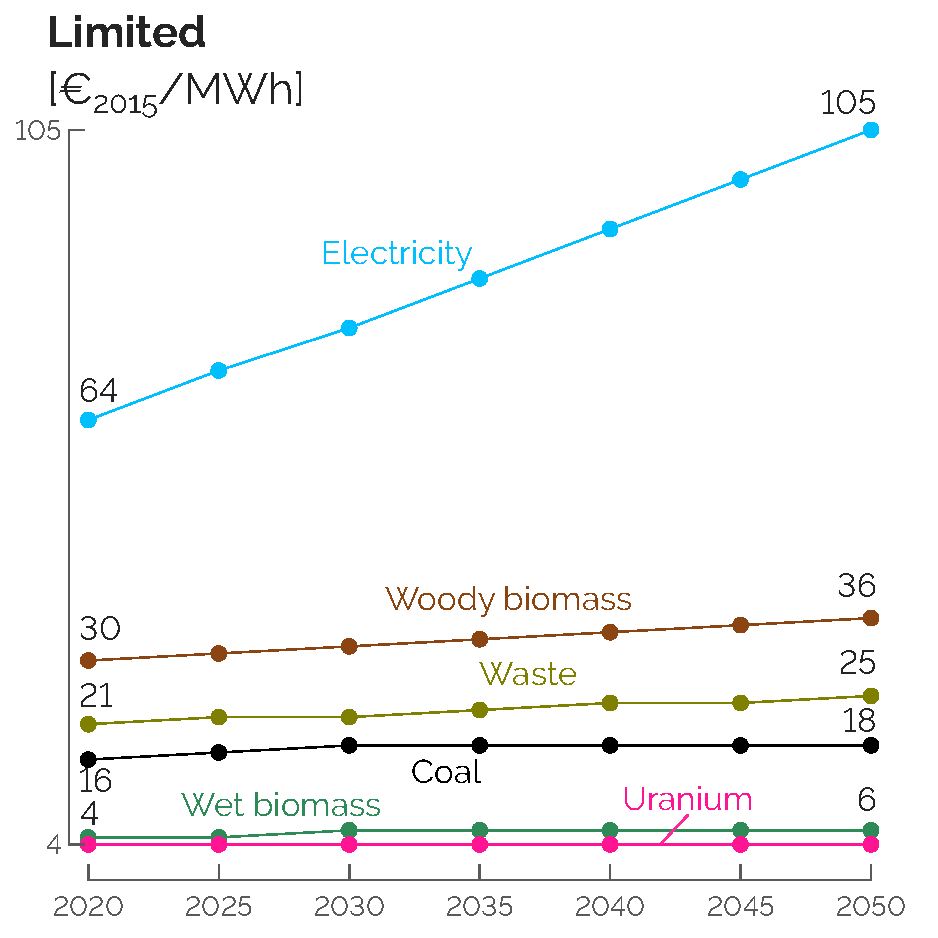
\includegraphics[width=0.32\textwidth]{Res_others.pdf}
\caption{Cost of purchasing the different resources. Besides the free local renewables (\ie sun, wind and hydro) limited by technical potentials, EnergyScope accounts for renewable energy carriers and their respective fossil counterparts (left and center graphs). These fuels can be imported from abroad without limitation on their availability. Other carriers are limited either by their local potentials (\ie biomass and waste) or other considerations like the power grid interconnections or the capacity of nuclear power plants.}
\label{fig:cs_resources_cost}
\end{figure}


\section{Conversion technologies: SMR, \gls{NED}-related and others}
\label{sec:cs:technologies}
As the end-use demands are defined as energy (and non-energy with the \gls{NED}) services rather than a certain quantity of oil or solar irradiance, for instance, technologies are implemented to convert these resources into the end-use demands. Besides their CAPEX, OPEX and lifetime defined in Section \ref{subsec:meth:ES_Pathway}, production and conversion technologies (\ie \gls{CCGT}, car or boiler) have a conversion efficiency whereas storage technologies (\ie thermal storage, battery or molecule storage) exhibit their own charge/discharge losses. Eventually, there are also infrastructure technologies like the grid or the \gls{DHN} that allow to account for the investment necessary, respectively, to integrate more intermittent renewables in the power sector and the expand the use of centralised heating systems. The exhaustive list of these technologies have already been presented in previous works \cite{limpens2021generating}.\\

A specific attention is to put on the implementation of \glsxtrfull{SMR} whereas the 6\,GW of conventional nuclear are assumed to drop to 2\,GW in 2025 and total phase-out by 2035. Similarly to the analysis of \citet{PATHS2050}, a Belgian consortium for energy research, and in line with the Belgian Nuclear Research Centre (SCK-CEN) \cite{SCK-CEN_SMR}, \gls{SMR} are implemented with the features listed in \Cref{tab:SMR_features}. Where most of the features are similar to conventional nuclear power plants, it differs from these on two main points: their potential year start, 2040, and their flexibility. Indeed, unlike the current nuclear power plants, constrained in the model to produce a constant power output at every hour of the year (\ie baseload production as it is actually the case in Belgium), SMRs, are flexible in the sense that their production can vary between 0 and their full capacity independently at any hour of each representative year. Here, we simplify SMRs as only producing electricity and assume that the after-heat is lost to the atmosphere anyway.


\begin{table}[htbp!]
\caption{Nominal features of the SMRs in EnergyScope. \gls{SMR} exhibits the advantage to have a fully flexible production (\ie between 0 to the full capacity) unlike conventional nuclear that is constrained to produce a constant baseload at every hour of the year. $^{(a)}$ This annual availability accounts for yearly maintenance where the reactors might not operate or, at least, not at their maximum capacity. $^{(b)}$ 2040 is the soonest year at which \gls{SMR} could be available, optimistically assuming industrial prototypes being completed by 2035 and 5 additional years for their commercial installation.}
\label{tab:SMR_features}
\centering
\begin{tabular}{l c c|c}
\toprule
\multirow{2}{*}{\textbf{Feature}} & \multirow{2}{*}{\textbf{Value}} & \multirow{2}{*}{\textbf{Unit}} & \textbf{Similarity with}\\
 & & & \textbf{conventional nuclear}\\
\midrule
CAPEX & 4850 & €/kW & \checkmark\\
Annual OPEX & 103 & €/kW/year & \checkmark\\
Lifetime & 60 & year & \checkmark\\
Efficiency & 40\% & -& \checkmark\\
Maximum capacity & 6 & GW & \checkmark\\
Annual availability & 85\%$^{(a)}$ & -& \checkmark\\
\midrule
Operational year & 2040$^{(b)}$ & - & \xmark\\
Flexibility & Full & - & \xmark\\
\bottomrule							

\end{tabular}
\end{table}

For the sake of comparison, \Cref{fig:LCOE} gives the \gls{LCOE} of the principal technologies to produce electricity, based on the computation used by \citet{limpens2021generating}. Compared to the other flexible generation units, \gls{SMR} is significantly more cost-effective. In addition, we see that \gls{CCGT} supplied by e-ammonia outcompetes its e-methane equivalent, unlike their respective fossil-based equivalent.

\begin{figure}[htbp!]
\centering
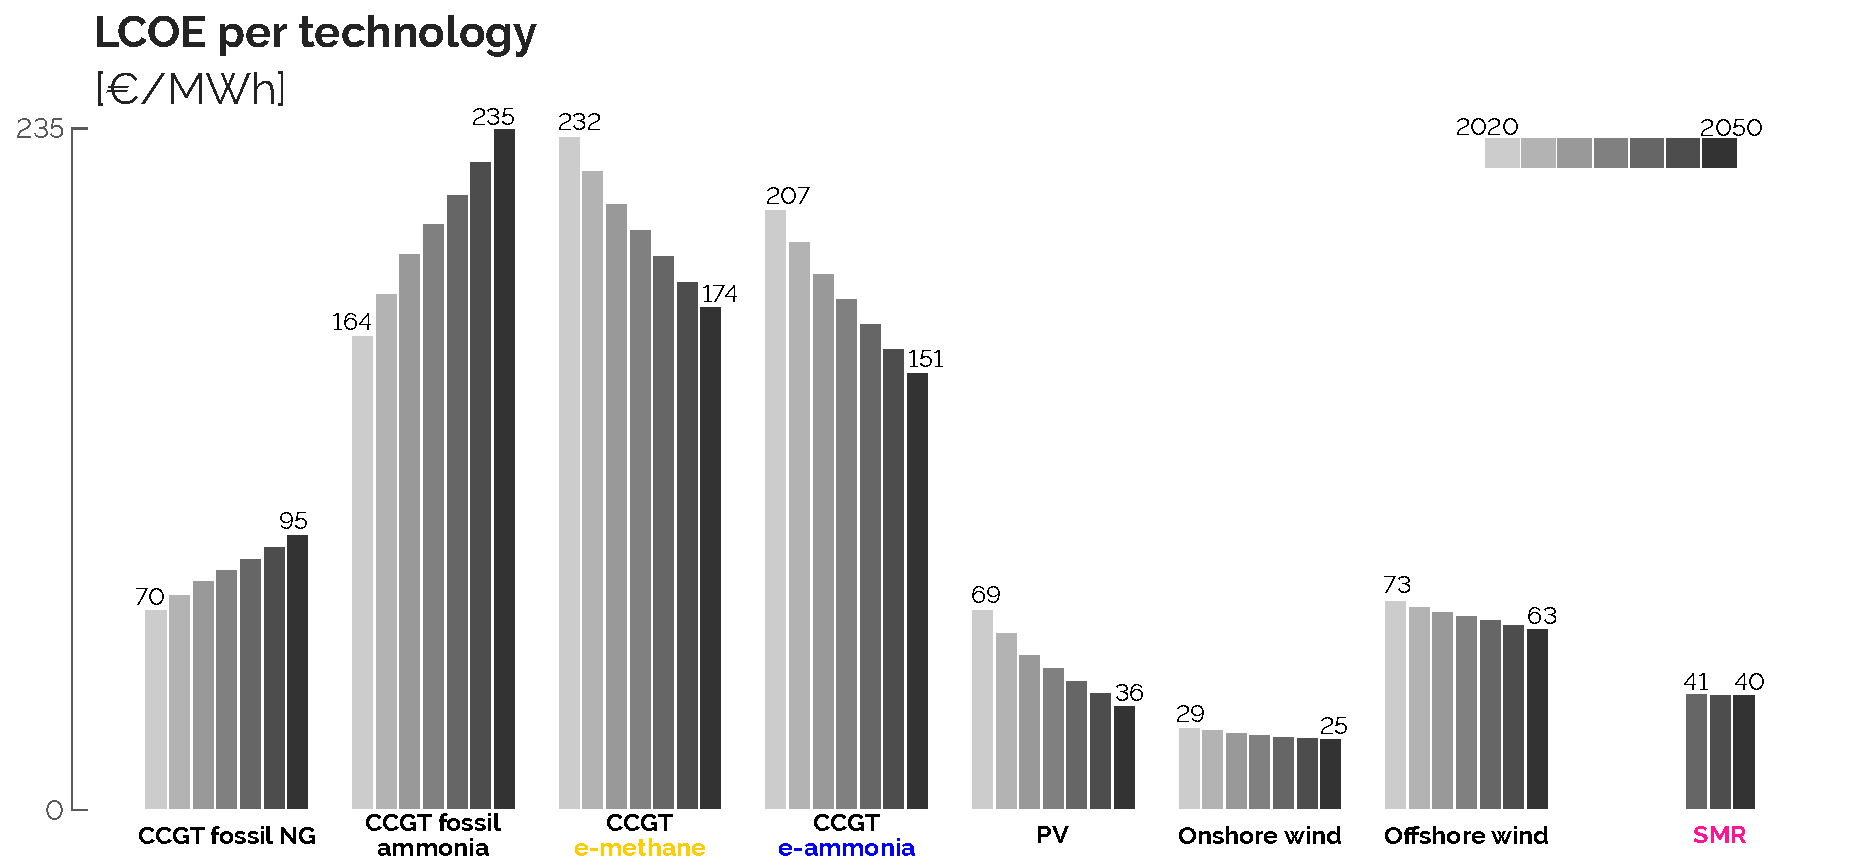
\includegraphics[width=0.8\textwidth]{LCOE.pdf}
\caption{Levelised cost of energy (LCOE) for the main technologies in the power sector. Where \gls{SMR} is cheaper than the other flexible options, CCGT running on e-ammonia is, a priori, cheaper than its e-methane alternative.}
\label{fig:LCOE}
\end{figure}

\autoref{fig:NED_tech} illustrates the different paths to produce the final molecules of the NED integrated within the model. Similarly to \cite{tsiropoulos2018emerging}, naphtha, here considered as \gls{LFO}, resulting from refinery operation is modeled as an imported commodity. Presented here for the specific year of 2035, all data and related references can be found in \cite{GIT_NED}. To keep the same level of details with other sectors of the model, the implementation of the conversion technologies consists of a single kind of technology per type of resource to produce a certain product. For instance, in the model, there is only one technology to produce \gls{HVC} either from naphtha or from LPG, two liquid fossil hydrocarbons, \ie \gls{NSC}. For ammonia and methanol, the molecules can either be produced locally from other resources or directly imported (with distinction between non-renewable and renewable molecules). Some other technologies included in the model (not represented here for the sake of clarity), are able to turn some resources presented here into others (\eg \gls{NG} to hydrogen, woody biomass to hydrogen or to synthetic natural gas, more information in \cite{Limpens2020}).

\begin{figure}[htbp!]
\centering
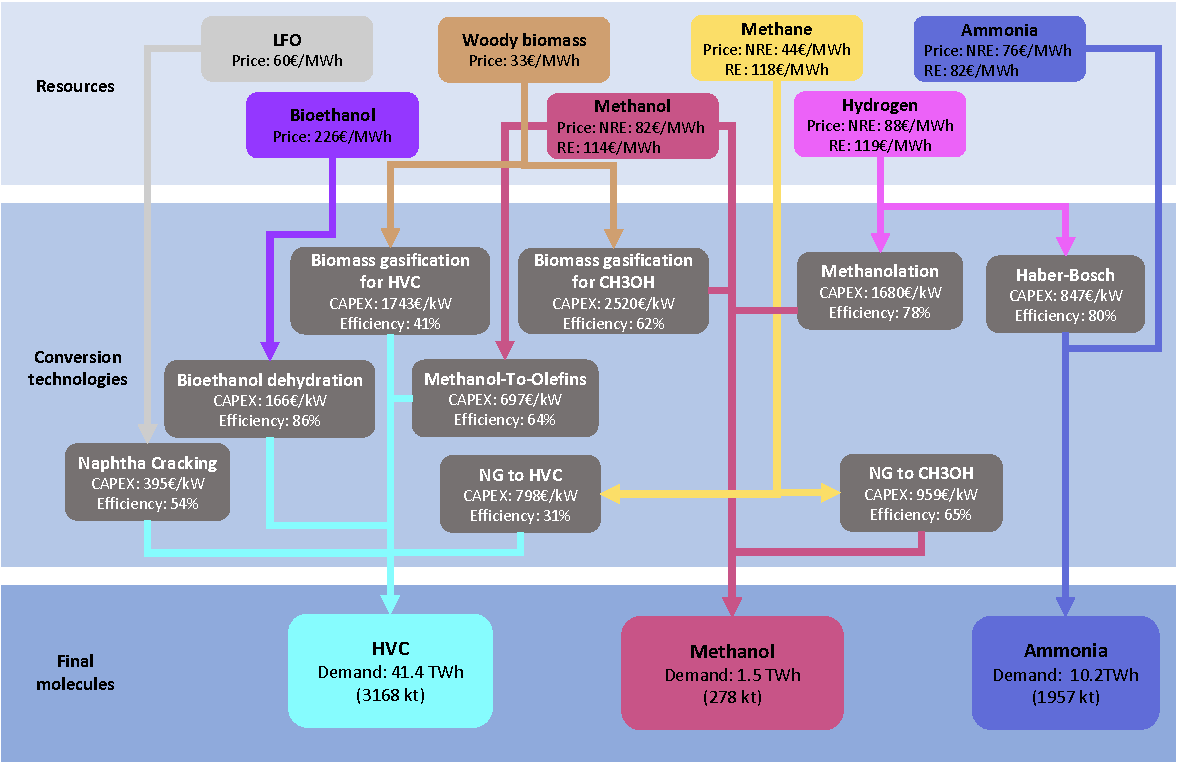
\includegraphics[width=0.8\textwidth]{NED_tech.pdf}
\caption{Schematic view of the different resources able to produce \gls{HVC}, ammonia and methanol with their related conversion technologies (including energy efficiency and their CAPEX - in €/kW of final molecules).  Values stand for 2035. Graph from \cite{rixhon2021comprehensive}}
\label{fig:NED_tech}
\end{figure}

\section{Uncertainty ranges}
\label{sec:cs:uncertainty}
\Cref{tab:UC_short} gives the uncertainty ranges of some key parameters. Like other works \cite{li2019renewables,coppitters2021robust}, the uncertain parameters are assumed to be independent and uniformly distributed between their respective lower and upper bounds. A particular attention is to pay to the potential installation of \gls{SMR}, at the bottom of \Cref{tab:UC_short}. As detailed before, the commercial availability of such a technology is uncertain but would not be before 2040. Consequently, for \gls{SMR}, the parameter $f_{\mathrm{max,SMR}}$ influences the maximum capacity to install to translate somehow the readiness of this technology. As SMRs are foreseen, if installed, to be around the same locations (\ie Tihange and Doel) as the conventional nuclear power plants and using the same area in kW/ha, the same 6\,GW are assumed to be the maximum capacity for SMRs. If it is (i) smaller than 0.6, there is no possibility to install \gls{SMR} during the transition; (ii) between 0.6 and 0.8, these 6~GW can be installed only in 2050; (iii) between 0.8 and 0.9, these can be installed from 2045 onward and; (iv) higher than 0.9, the prescribed maximum capacity can be installed from 2040 onward. Based on the local sensitivity analysis carried out by \citet{PATHS2050}, the current work also considers a [-40\%; +44\%] range on the CAPEX of SMR, on top of the uncertainty about the availability. Finally, the the cost of purchasing renewable electrofuels presents a wide range, [-64.3\%; +179.8\%], like the other imported commodities.

The exhaustive list of the parameters accounted in this work is presented in Appendix \ref{app:UC_full}.

\begin{table}[htbp!]
\caption{Illustration of the uncertainty characterisation for different parameters for the year 2025. $^{(a)}$ Per \cite{Moret2017PhDThesis}, \og I: investment-type, II: operation-type (constant uncertainty over time), III: operation-type (uncertainty increasing over time)\fg. $^{(b)}$ The nominal value of each parameter is 0, meaning no variation compared to the nominal values of the impacted parameter in the model. $^{(c)}$ This range has been inferred from the local sensitivity analysis performed by \citet{PATHS2050}.}
\label{tab:UC_short}
\centering
\resizebox{\textwidth}{!}{
\begin{tabular}{l l l c c c}
\toprule
\multirow{2}{*}{\textbf{Category}} & \multirow{2}{*}{\textbf{Parameter}} & \multirow{2}{*}{\textbf{Meaning}} & \multirow{2}{*}{\textbf{Type}$^{(a)}$}  & \multicolumn{2}{c}{\textbf{Relative variation$^{(b)}$}}\\
    & & & &	 min 	&	 max \\ 	
\midrule		
\multirow{2}{*}{\textbf{Cost of purchasing}} & $c_{\mathrm{op,fossil}}$ & Purchase fossil fuels & II & -64.3\% & 179.8\% \\
& $\bm{c_{\mathrm{op,electrofuels}}}$ & \textbf{Purchase electrofuels} & \textbf{II} & \textbf{-64.3\%} & \textbf{179.8\%} \\
\midrule
\multirow{5}{*}{\textbf{Investment cost}} &$c_{\mathrm{inv,car}}$ & CAPEX car  & I & -21.6\% & 25.0\% \\
& $c_{\mathrm{inv,e\_prop}}$ & CAPEX electric motor & I & -39.6\% & 39.6\% \\
& $c_{\mathrm{inv,fc\_prop}}$ & CAPEX fuel cell engine & I & -39.6\% & 39.6\% \\
& $c_{\mathrm{inv,PV}}$ & CAPEX PV & I & -39.6\% & 39.6\% \\
& $\bm{c_{\mathrm{inv,nuclear\_SMR}}}$ & \textbf{CAPEX \gls{SMR}}$^{(c)}$ & \textbf{I} & \textbf{-40.0\%} & \textbf{44.0\%} \\
\midrule
\multirow{1}{*}{\textbf{Consumption}} &$\eta_{\mathrm{e\_prop}}$ & Consumption electric vehicles & I & -28.7\% & 28.7\% \\
\midrule
\multirow{2}{*}{\textbf{Potential installed capacity}} &$f_{\mathrm{max,PV}}$ & Max capacity PV & I & -24.1\% & 24.1\% \\
& $f_{\mathrm{max,windon}}$ & Max capacity onshore wind & I & -24.1\% & 24.1\% \\
\midrule
\multirow{2}{*}{\textbf{Hourly load factor}} & $c_{\mathrm{p,t,PV}}$ & Hourly load factor PV & II & -22.1\% & 22.1\% \\
& $c_{\mathrm{p,t,winds}}$ & Hourly load factor wind turbines & II & -22.1\% & 22.1\% \\
\midrule
\multirow{2}{*}{\textbf{Resource availability}} & $avail_{\mathrm{elec}}$ & Available electricity import & I & -32.1\% & 32.1\% \\
& $avail_{\mathrm{biomass}}$ & Available local biomass & I & -32.1\% & 32.1\% \\
\midrule

\multirow{2}{*}{\textbf{End-use demand}} & $pass\_EUD$ & Passenger mobility EUD & III & -7.5\% & 7.5\% \\
& $industry\_EUD$ & Industry EUD & III & -20.5\% & 16.0\% \\
\midrule

\multirow{4}{*}{\textbf{Miscellaneous}} &$i_{\mathrm{rate}}$  & Interest rate & I & -46.2\% & 46.2\% \\
& $\Delta_{\mathrm{change,freight}}$ & Modal share change freight mobility & - & -30\% & 30\% \\
& $\Delta_{\mathrm{change,pass}}$ & Modal share change passenger mobility & - & -30\% & 30\% \\
& $\bm{f_{\mathrm{max,SMR}}}$ & \textbf{Potential capacity \gls{SMR}} & \textbf{-} & \textbf{0} & \textbf{1} \\

\bottomrule							

\end{tabular}}
\end{table}

\section{\ce{CO2}-budget for the transition}
\label{sec:cs:CO2-budget}
In most of the studies carried out on the pathway optimisation of a whole-energy system, a \ce{CO2}-trajectory is \textit{a priori} set to reach carbon-neutrality by 2050. \citet{nerini2017myopic} used the emission trajectory indicated by the UK's Committee on Climate Change in their analysis of the impact of limited foresight to achieve the target of 80\% reduction of \gls{GHG} by 2050 in the United Kingdom. In their assessment of the impacts of economy-wide emissions policies in the water-energy-land nexus, \citet{licandeo2023assessing} analysed different \ce{CO2}-trajectories considering more or less severe water scarcity for the US. \citet{poncelet2016myopic} with LUSYM (Leuven University SYstem Model) and \citet{PATHS2050} with TIMES-BE also set decreasing emission trajectories in their analysis of respectively the Belgian power sector and whole-energy system.  Others only set the objective as the carbon-neutrality by 2050. For instance, \citet{heuberger2018impact} investigated the impact of different factors (\eg limit of the foresight in the future, availability of \og unicorn technologies\fg or committed versus market-driven decarbonisation strategies) to reach this ultimate objective in the UK system.\\

In this work, the effect of greenhouse gases is cumulative over time and a constraint is set on the overall emissions of the transition---a \ce{CO2}-budget for the transition. The arbitrarily chosen way of attributing emissions-budget to Belgium is usually called \og grandfathering\fg. Even though this approach has his pros and cons out of discussion within the scope of this work, it consists in \og maintaining that prior emissions increase future emission entitlements\fg \cite{knight2013grandfathering}. This budget (1.2\,Gt$_{\ce{CO2},\text{eq}}$) corresponds to the proportion of Belgium's emissions in the world emissions in 2020 (34.8\,Gt$_{\ce{CO2},\text{eq}}$ \cite{ourworldindata_CO2_world}) applied to the global budget to have a 66\% chance of limiting warming to 1.5°C of 420\,Gt$_{\ce{CO2},\text{eq}}$ \cite{IPCC_CO2_budget}. Therefore, in this work, a limit has been put on $\emph{gwp\textsubscript{lim,trans}}=1.2\,\text{Gt}_{\ce{CO2},\text{eq}}$ in Eq.\,(\ref{eq:limit_gwp_trans}). This is another sign of the urgency to act to mitigate climate change as this 30-year budget represents only 10 years of the current emissions. \\

Compared to a linear decrease from the current emissions, as done by \citet{limpens2024pathway}, this budget represents a 60\% reduction of the cumulative emissions over the transition.  Appendix \ref{app:CO2_budget} compares the emissions trajectory between the REF case and a case (without \gls{SMR}) where the linear decrease is imposed between 2020 and carbon-neutrality in 2050.